\documentclass[a4paper,10pt]{extarticle}
\usepackage[a4paper]{geometry}
\geometry{verbose,tmargin=2cm,bmargin=2cm,lmargin=2cm,rmargin=2cm}

\usepackage{fontspec}
\setmonofont{FreeMono}

\setlength{\parindent}{0cm}
\setlength{\parskip}{0.5em}

\usepackage{textcomp}
\usepackage{graphicx}
\usepackage{hyperref}
\usepackage{url}
\usepackage{xcolor}

\usepackage{minted}
\newminted{python}{breaklines,fontsize=\small}
\newminted{text}{breaklines,fontsize=\small}

\definecolor{mintedbg}{rgb}{0.95,0.95,0.95}
\usepackage{mdframed}

\BeforeBeginEnvironment{minted}{\begin{mdframed}[backgroundcolor=mintedbg]}
\AfterEndEnvironment{minted}{\end{mdframed}}

\title{
Tugas Kelompok \\
MI3103 - Antar Muka Komputer}
\author{}
\date{}

\begin{document}
\maketitle

\textbf{Soal 1}

Buatlah program Python (dengan pustaka Numpy dan Matplotlib)
untuk membuat histogram dari dua distribusi bilangan
acak Gaussian dengan parameter $(\mu,\sigma) = (-0.2,0.25)$
dan $(\mu,\sigma) = (0.35,0.3)$.

Hasil plot yang Anda buat seharusnya terlihat seperti berikut.

\begin{figure}[h]
{\centering
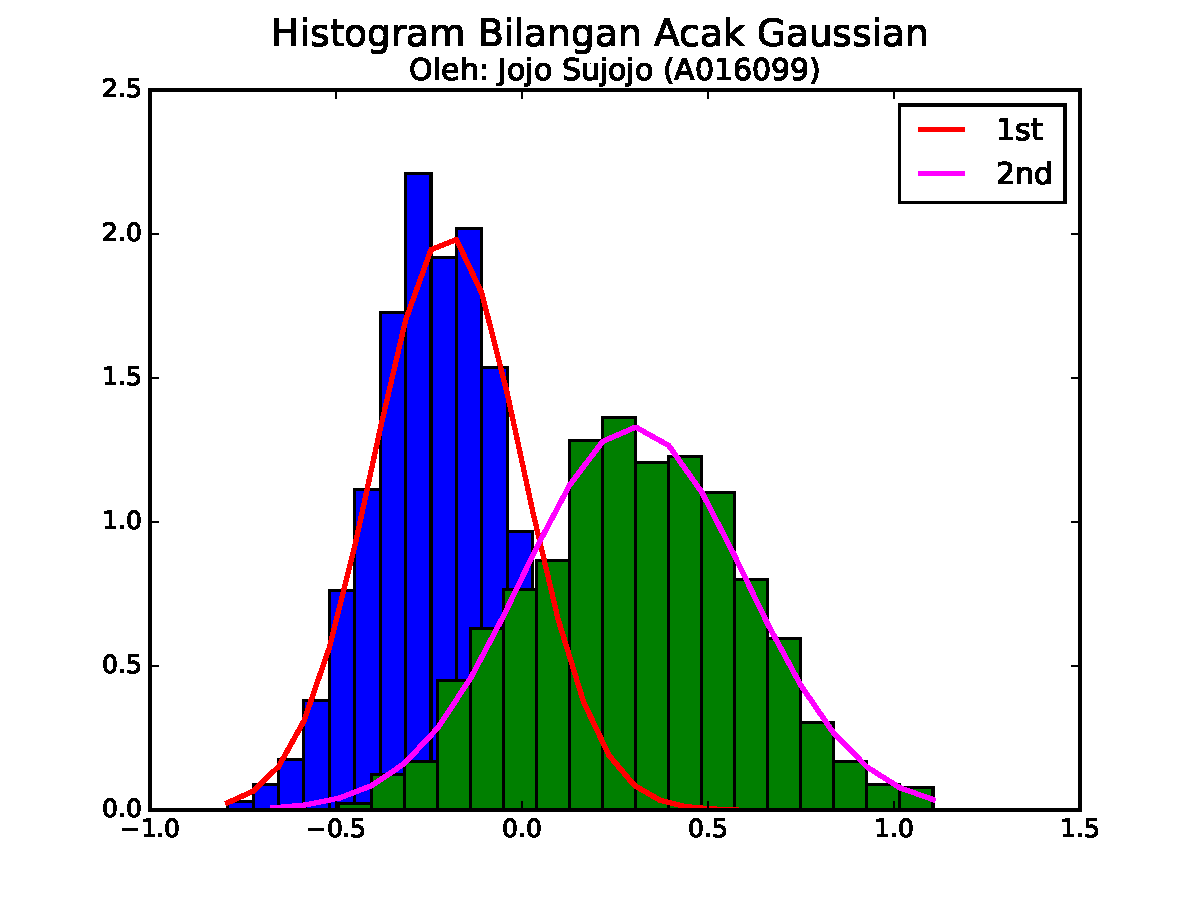
\includegraphics[scale=0.5]{images/normal_v1.pdf}
\par}
\end{figure}
%
Plot yang Anda buat harus tertera nama beserta NIM Anda (seperti contoh).

\textbf{Soal 2}

Buatlah kode (HTML + Javascript) dengan spesifikasi sebagai berikut.
\begin{itemize}
\item Halaman dengan form sederhana yang meminta nama dan NIM Anda beserta
button Submit/OK.
\item Ketika button Submit/OK ditekan, browser akan menampilkan alert box
dengan nama dan NIM Anda.
\end{itemize}

\begin{figure}[!h]
{\centering
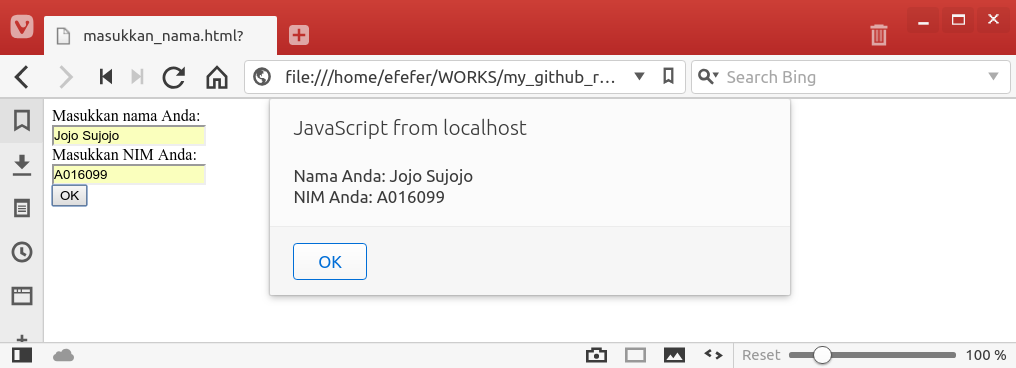
\includegraphics[scale=0.4]{images/JojoSujojo.png}
\par}
\end{figure}

\textbf{Soal 3}

Buatlah program Flask sederhana untuk merespon permintaan seperti berikut ini:
\begin{textcode}
http://localhost:5000/process-data?nama=Jojo&makanan=Nasi%20Tumpeng&minuman=Teh%20susu
\end{textcode}
Dan memberikan respon di \textit{browser}
berupa teks (atau dalam HTML yang diformat dengan baik):
\begin{textcode}
Detail pesanan
Nama : Jojo
Makanan : Nasi Tumpeng
Minuman : Teh susu
Pesanan Anda telah diterima pada 2018-12-04 11:19:27.593624 
\end{textcode}

\textbf{Soal 4}

Mirip seperti dalam soal sebelumnya, namun dengan menggunakan HTML form.
User akan diminta mengisi tiga data seperti soal sebelumnya
yaitu nama, makanan, dan minuman serta alamat pengiriman.
Gunakan metode POST untuk meng-handle permintaan tersebut.

\textbf{Soal 5}

Dalam bagian ini kita akan membuat suatu aplikasi web sederhana
yang mampu menerima data pengukuran dan menampilkannya di browser.
Kita tidak menggunakan data pengukuran sebenarnya, namun akan menggunakan
script Python sederhana sebagai simulasi pengiriman data dari alat pengukuran.
Misalkan script tersebut bernama \verb|send_data.py|.
\begin{pythoncode}
import numpy as np
import time
import requests

def gen_rand_data(minT, maxT, prec=50):
    deltaT = (maxT - minT)/prec
    return minT + (np.random.randint(1,prec+1)-1)*deltaT

while True:
    dat_T = gen_rand_data(30,50)
    print("Sending data by GET method ...")
    rec_str = "http://localhost:5000?data=" + str(dat_T)
    requests.get(rec_str)
    time.sleep(1.0)
\end{pythoncode}

Untuk menjalankan kode ini, server Flask pada \url{http://localhost}
harus sudah berjalan sebelumnya. Anda dapat melakukan ini dengan cara,
misalnya, menjalankan server Flask (dengan \texttt{flask run} atau cara
alternatif) kemudian menjalankan \texttt{python send\_data.py} pada
terminal lain.

\begin{enumerate}
\item Berikan penjelasan mengenai kode yang ada pada \verb|send_data.py| di atas.
\item Desainlah aplikasi web sederhana dengan menggunakan Python + Flask untuk
menerima data dari \verb|send_data.py|. Untuk aplikasi sederhana ini, Anda dapat
menyimpan data yang diterima dalam file teks saja. 
Data tersebut terdiri dari dua kolom, yaitu waktu data diterima dan nilai (numerik)
dari data tersebut.
Kemudian buat juga link, misalnya \url{http://localhost:5000/show-data},
untuk menampilkan visualisasi data tersebut pada browser
(boleh menggunakan \textsf{Plotly.js} atau pustaka lain).
\item Pada kode di atas kita telah menggunakan metode GET untuk mengirimkan data.
Jelaskan apa yang harus dilakukan jika kita ingin menggunakan metode POST?
\end{enumerate}


\end{document}


